\documentclass{article}
\usepackage{pdfpages}
\usepackage{enumitem}
% Language setting
% Replace `english' with e.g. `spanish' to change the document language
\usepackage[english]{babel}

% Set page size and margins
% Replace `letterpaper' with `a4paper' for UK/EU standard size
\usepackage[letterpaper,top=2cm,bottom=2cm,left=3cm,right=3cm,marginparwidth=1.75cm]{geometry}

% Useful packages
\usepackage{amsmath}
\usepackage{graphicx}
\usepackage[colorlinks=true, allcolors=blue]{hyperref}

\title{Electrónica Industrial - Trabajo Práctico Teórico n° 9}
\author{Abel Corvalán - 41.220.050}
\date{}
\begin{document}
\maketitle
\section{Consignas}

\begin{enumerate}

\item Implementar el control de un motor de corriente continua para una cinta de caminar con los siguientes datos:

Tensión: 180 volt; corriente nominal: 4,2 A; Potencia: 1 HP, rpm: 4000

Tiene una correa para adecuar la velocidad final máxima de 10 km/h.


\begin{enumerate}[label=\alph*.]
    \item  Elegir el circuito de potencia más simple y el circuito de control apropiado para la aplicación. Explicar su funcionamiento. Calcular todos sus componentes asociados. Colocar hoja de datos.

    \item Dibujar el circuito completo.

    \item Simular el circuito final.
\end{enumerate}

\item Diseñar la placa de control de un semáforo con luces roja, amarillo y verde para lámparas de 120 W. Las lámparas son conectadas a 220 volt CA.

\begin{enumerate}[label=\alph*.]

    \item Utilizar optoacopladores y/o MOC para el diseño. Indicar en la placa con leds la operación de cada luz. La operación de cada luz se realiza a través de un microcontrolador (no hay que colocar el micro).

    \item Realizar la simulación del sistema.
\end{enumerate}
\end{enumerate}

\section{Desarrollo}

\begin{enumerate}
    \item Control de motor de corriente continua
\begin{enumerate}[label=\alph*.]
    \item Se propone la siguiente topología para el circuito de potencia:




El circuito se compone un rectificador de onda completa con un capacitor de filtro. Luego se tiene un transistor MOSFET el cual controla la tensión media que llega al motor mediante la modulación del canal por medio de tensiones en el pin Gate del dispositivo. 
Se coloca un diodo en paralelo a la carga debido a la componente inductiva que tiene el motor.

\begin{figure}[h!]
    \centering
    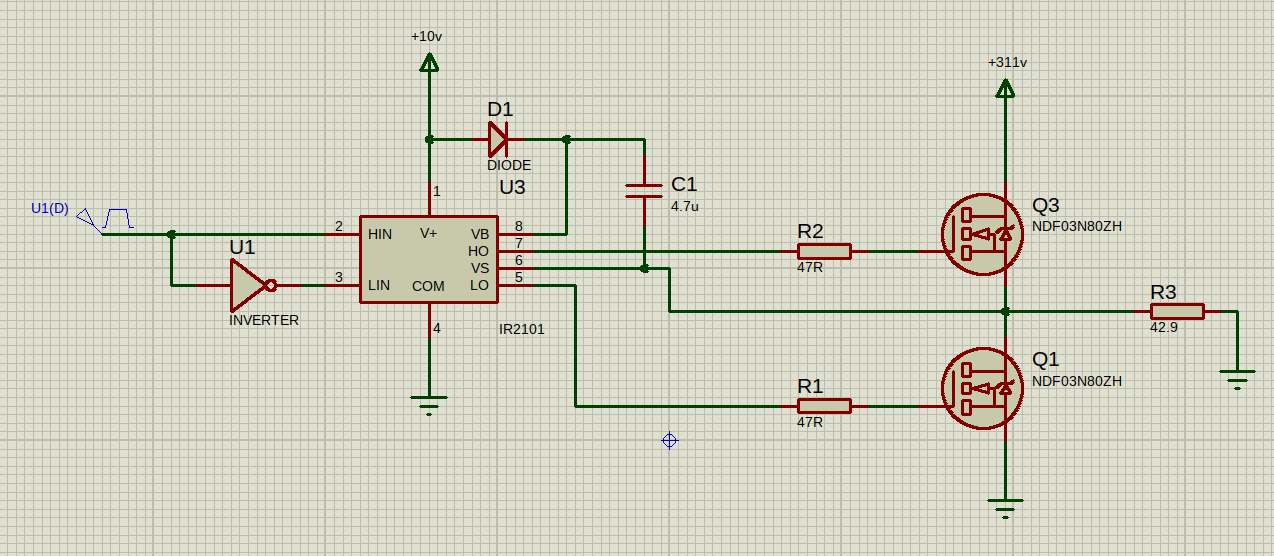
\includegraphics[width=0.6\linewidth]{img/Circuito para motor CC.png}
    \caption{Caracterísiticas del MOSFET SIHA17N80AEF}
    \label{fig:esquematico}
\end{figure}


%COMMENT


En primer instancia se calcula la resistencia de la carga:

$$ \boxed{ R_{L}= \frac{V_{nominal}}{I_{nominal}} } $$
$$ R_{L}= \frac{180V}{4.2A}= 42.857 \Omega \approx 42.9 \Omega $$
$$ \boxed{ R_{L}= 42.9 \Omega } $$
Se selecciona el transistor MOSFET con los siguientes datos:

$$ I_{DS_{calc}}= 4.2A \, 1.5= 6.3A $$
$$ \boxed{ I_{DS_{calc}}= 6.3A } $$
$$ V_{DS_{calc}}= 311V \, 2.5= 777.5V $$

Se selecciona el MOSFET modelo SIHA17N80AEF.

\begin{figure}[h!]
    \centering
    \includegraphics[width=0.6\linewidth]{img/Transistor MOSFET seleccionado.png}
    \caption{MOSFET modelo SIHA17N80AEF}
    \label{fig:esquematico}
\end{figure}
\begin{figure}[h!]
    \centering
    \includegraphics[width=0.6\linewidth]{img/Caracterísiticas MOSFET.png}
    \caption{Caracterísiticas del MOSFET SIHA17N80AEF}
    \label{fig:esquematico}
\end{figure}
Se realiza la selcción de los diodos rectificadores.

$$ I_{F(AV)}= \frac{I_{L(AV)}}{2}= \frac{4.2A}{2}= 2.1A $$
$$ I_{F(AV)_{calc}}= 2.1A \, 1.5= 3.15A $$
$$ \boxed{ I_{F(AV)_{calc}}= 3.15A } $$

$$ V_{RRM}= 311V \, 2.5= 777.5V $$
$$ \boxed{ V_{RRM}= 777.5V } $$

Se determina el ancho del pulso para obtener una caída de tensión en la carga de $ V_{L(AV)}= 180V $.

$$ Porcentaje_{Duty \, cycle}= \frac{180V}{311V}= 0.578 \approx 0.58 $$
$$ \boxed{ Porcentaje_{Duty \, cycle} \, (\%)= 58\% } $$

%Si quisieramos un sistema con mayor rendimiento respecto del consumo de potencia optaríamos por reducir la frecuencia de la señal que controla el MOSFET.






\end{enumerate}

\item Se diseña el circuito de control de un semáforo.

Se establece la siguiente secuencia de encendido de las luces del semáforo:

- Luz roja: 2 segundos \\  
- Luz amarilla: 1 segundo \\
- Luz verde: 3 segundos 

\end{enumerate}

\begin{enumerate}[label=\alph*.]
    \item Se implementa el modelo del optoacoplador MOC3031M.

\begin{figure}[h!]
    \centering
    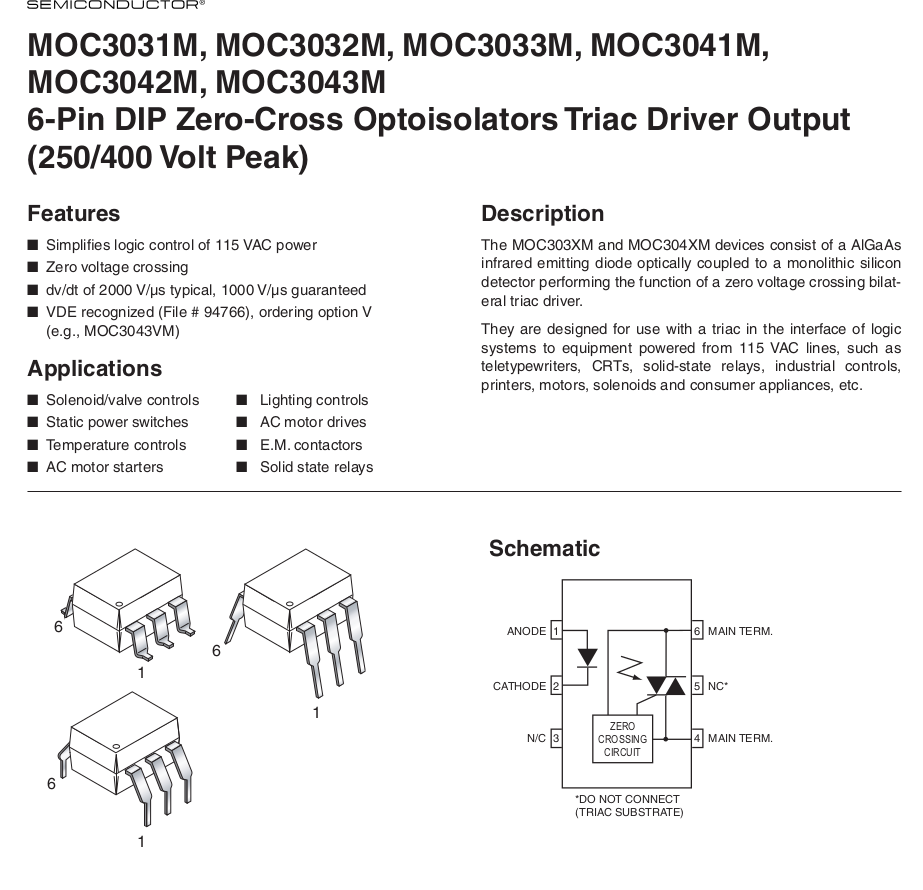
\includegraphics[width=0.6\linewidth]{img/MOC3031.png}
    \caption{Datasheet MOC3031}
    \label{fig:esquematico}
\end{figure}

\newpage

Se realiza su circuito de aplicación para las tres luces.

\begin{figure}[h!]
    \centering
    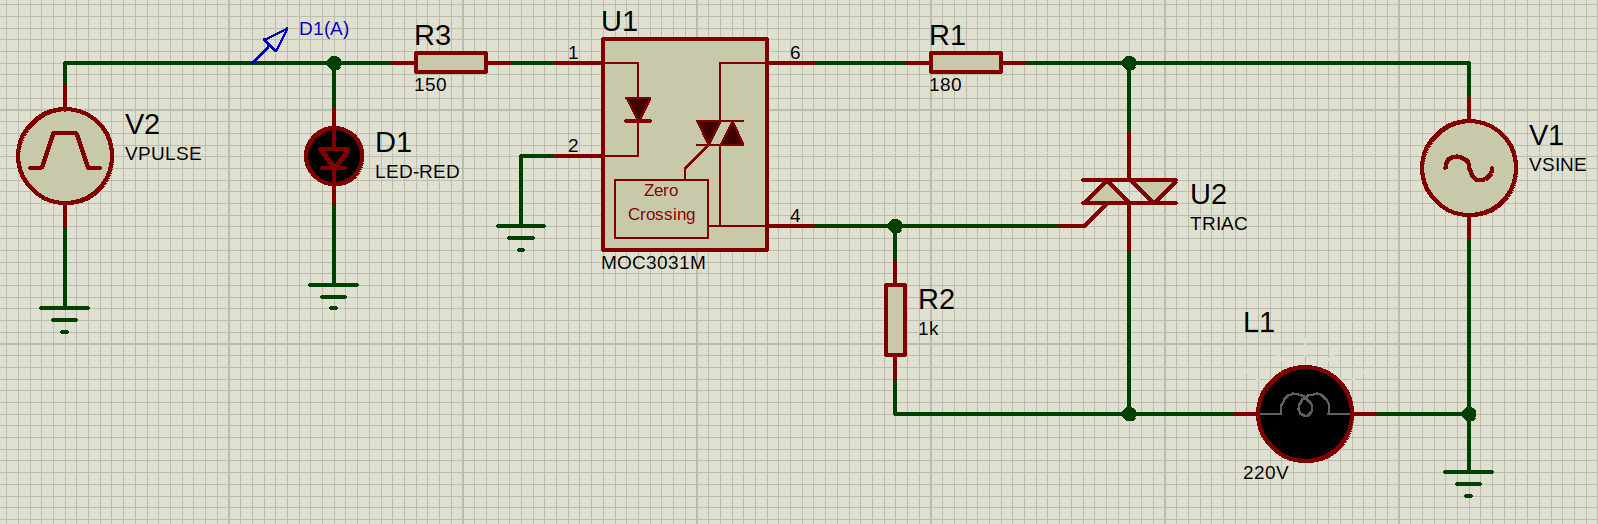
\includegraphics[width=0.6\linewidth]{img/Circuito de aplicación.png}
    \caption{Circuito de aplicación MOC3031M}
    \label{fig:esquematico}
\end{figure}

Se tiene como dato del dispositivo MO3031M que la corriente $I_{in}= 15mA$, por lo que se calcula la resistencia de entrada $R_{in}$ de la siguiente forma.

$$ R_{in}= \frac{V_{D}-V_{in \, MOC}}{I_{in \, MOC}}= \frac{5V-3V}{15mA}= 133 \Omega $$

Se coloca un valor comercial del mismo.

$$ \boxed{ R_{in}= 150 \Omega } $$

    \item Se realiza la simulación del sistema completo.

\begin{figure}[h!]
    \centering
    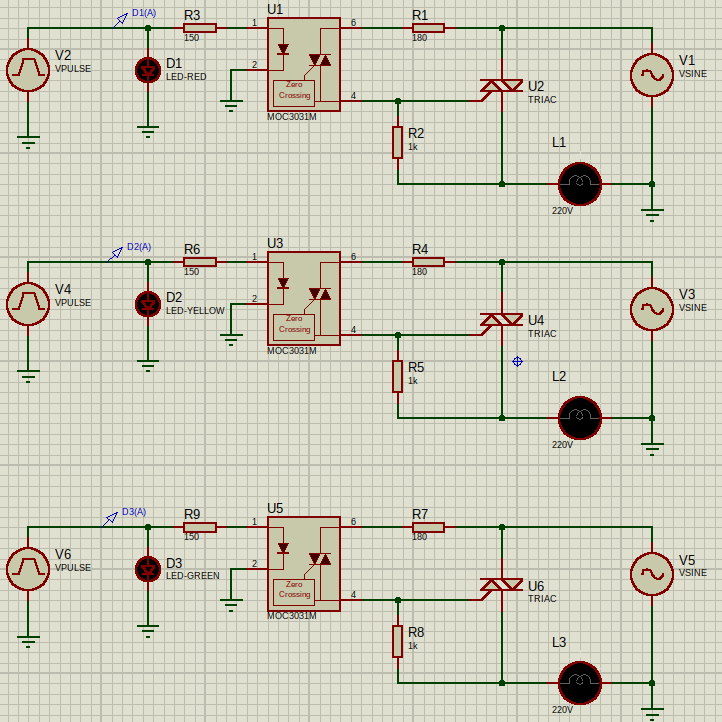
\includegraphics[width=0.6\linewidth]{img/Semaforo completo.png}
    \caption{Sistema de semáforo completo}
    \label{fig:esquematico}
\end{figure}

A continuación se muestra la secuencia del semáforo.

\begin{figure}[h!]
    \centering
    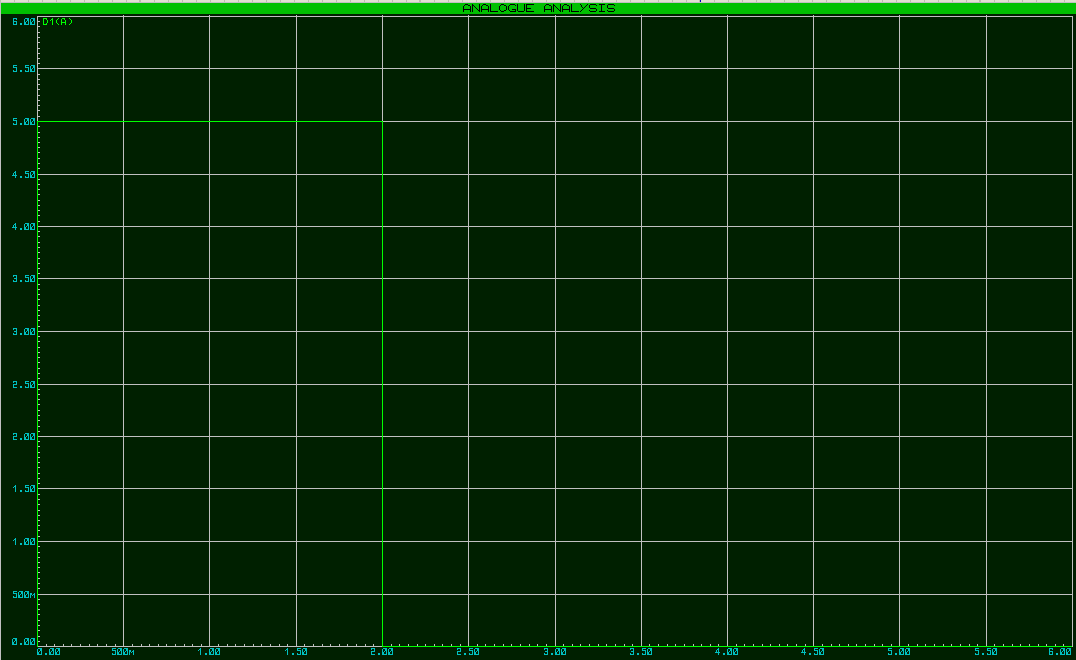
\includegraphics[width=0.6\linewidth]{img/Señal rojo.png}
    \caption{Luz roja}
    \label{fig:esquematico}
\end{figure}


\begin{figure}[h!]
    \centering
    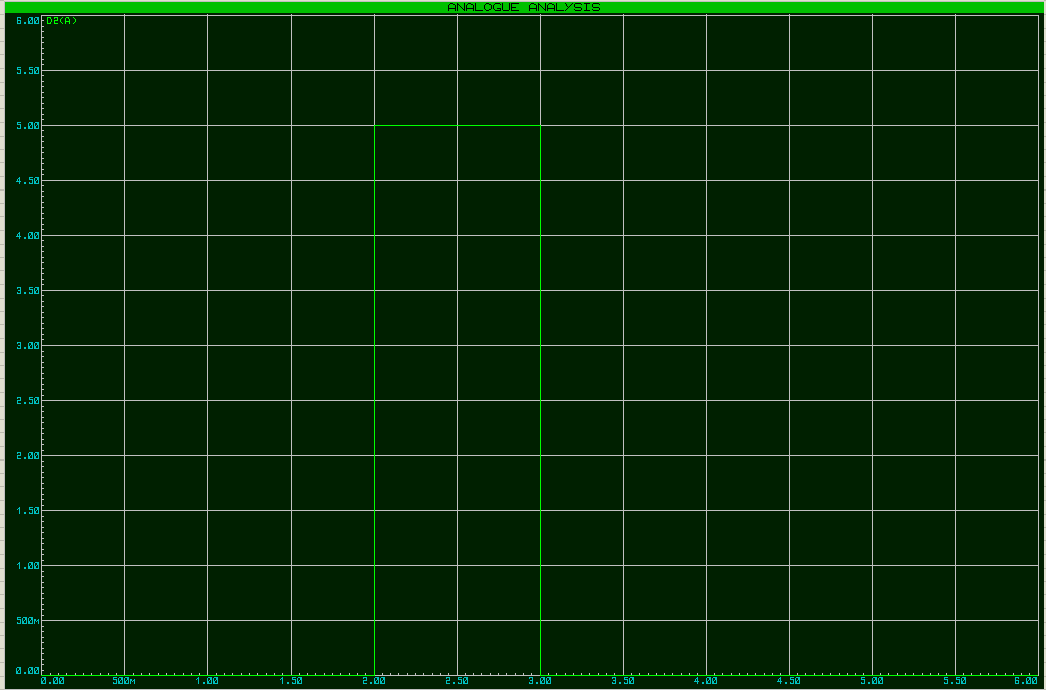
\includegraphics[width=0.6\linewidth]{img/Señal amarillo.png}
    \caption{Luz amarilla}
    \label{fig:esquematico}
\end{figure}

\begin{figure}[h!]
    \centering
    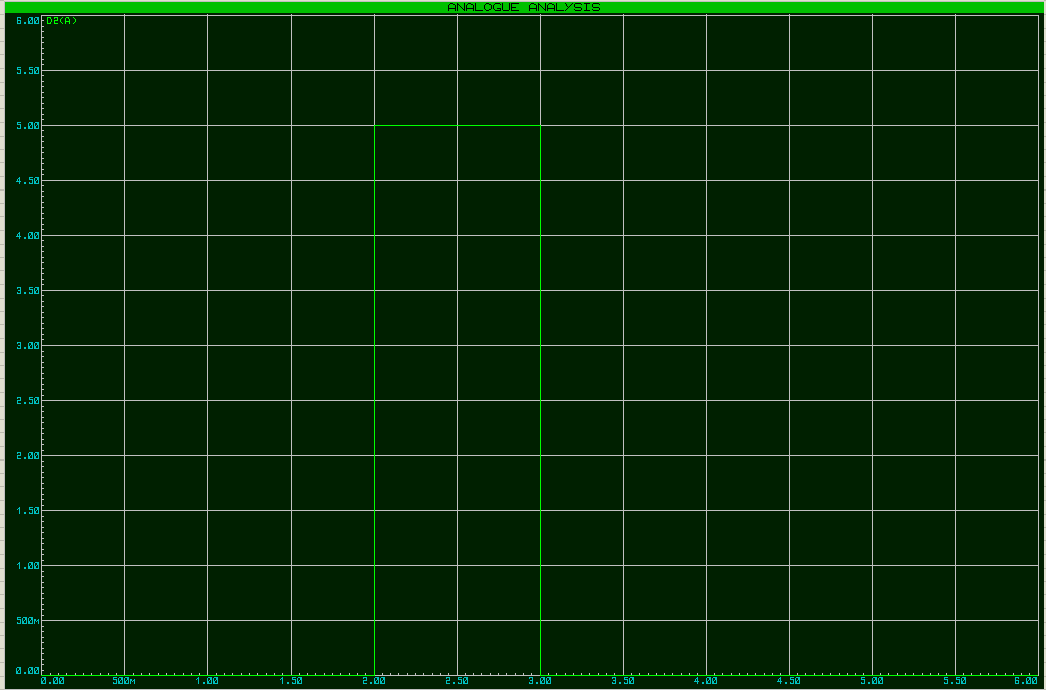
\includegraphics[width=0.6\linewidth]{img/Señal amarillo.png}
    \caption{Luz amarilla}
    \label{fig:esquematico}
\end{figure}

\end{enumerate}

\end{document}